\documentclass{article}
\usepackage[utf8]{inputenc}

\title{Tikz_example}
\author{kasperlaustsen }
\date{October 2021}

% \begin{document}
	% \documentclass{article}
	\usepackage{tikz}
	\usetikzlibrary{shapes,arrows,positioning,calc}
	
	\begin{document}
		
		\tikzset{
			block/.style = {draw, fill=white, rectangle, minimum height=3em, minimum width=3em},
			tmp/.style  = {coordinate}, 
			sum/.style= {draw, fill=white, circle, node distance=1cm},
			input/.style = {coordinate},
			output/.style= {coordinate},
			pinstyle/.style = {pin edge={to-,thin,black}
			}
		}
		
		
		
		\begin{figure}[!htb]
%			\centering
				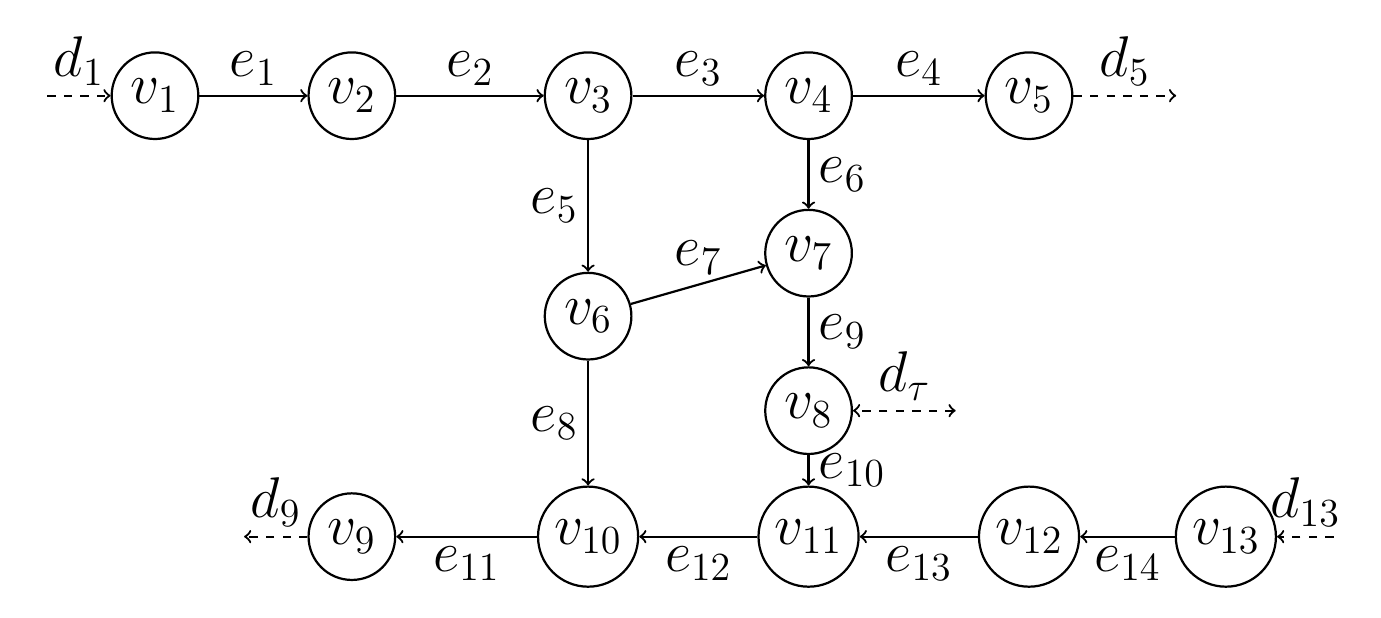
\begin{tikzpicture}[node distance=28mm, thick, main/.style = {draw,circle,minimum size=1.1cm}] 
					\node (1)  {};
					\node[main] (2) [node distance={15mm},right of=1] {\huge $v_1$}; 
					\node[main] (3) [node distance={2.5cm},right of=2] {\huge $v_2$};
					\node[main] (4) [node distance={3cm},right of=3] {\huge $v_3$};
					\node[main] (5) [right of=4] {\huge $v_4$};
					\node[main] (6) [right of=5] {\huge $v_5$};
					\node (7) [node distance={20mm},right of=6] {};
					%Create 3 (4) nodes in middle part of graph
					\node[main] (8) [below of=4] {\huge $ v_6 $};
					\node[main] (9) [node distance={20mm},below of=5] {\huge $ v_7 $};
					\node[main] (11) [node distance={20mm},below of=9] {\huge $ v_8 $};
					\node (10) [node distance={20mm},right of=11] {};
					%First 5 (7) nodes in bottom part of graph
					\node[main] (12) [below of=8] {\huge $ v_{10} $};
					\node[main] (13) [node distance = {3cm},left of=12] {\huge $ v_9 $};
					\node(14) [node distance={15mm},left of=13] {};
					\node[main] (15) [right of=12] {\huge $ v_{11} $};
					\node[main] (16) [right of=15] {\huge $ v_{12} $};
					\node[main] (17) [node distance={2.5cm},right of=16] {\huge $ v_{13} $};
					\node(18) [node distance={15mm},right of=17] {};
					
					%Edges with direction
					\path [->] (2) edge node[above] {\huge $e_{1}$} (3); 	%Edge v1 -> v2
					\path [->] (3) edge node[above] {\huge $e_{2}$} (4); 	%Edge v2 -> v3
					\path [->] (4) edge node[above] {\huge $e_{3}$} (5); 	%Edge v3 -> v4
					\path [->] (5) edge node[above] {\huge $e_{4}$} (6); 	%Edge v4 -> v5
					
					\path [->] (4) edge node[left] {\huge $e_{5}$} (8); 	%Edge v3 -> v6
					\path [->] (5) edge node[right] {\huge $e_{6}$} (9); 	%Edge v4 -> v7
					\path [->] (8) edge node[above] {\huge $e_{7}$} (9); 	%Edge v6 -> v7
					\path [->] (8) edge node[left] {\huge $e_{8}$} (12); 	%Edge v6 -> v10
					\path [->] (9) edge node[right] {\huge $e_{9}$} (11); 	%Edge v7 -> v8
					\path [->] (11) edge node[right] {\huge $e_{10}$} (15);	 %Edge v8 -> v11
					
					
					\path [->] (12) edge node[below] {\huge $e_{11}$} (13); %Edge v10 -> v9
					\path [->] (15) edge node[below] {\huge $e_{12}$} (12); %Edge v11 -> v10
					\path [->] (16) edge node[below] {\huge $e_{13}$} (15); %Edge v12 -> v11
					\path [->] (17) edge node[below] {\huge $e_{14}$} (16); %Edge v13 -> v12
					
					%External flows
					\draw[->,dashed,] (1) -- node[above] {\huge $d_1$} (2); %Create d1
					\draw[->,dashed,] (6) -- node[above] {\huge $d_5$} (7); %Create d5
					\draw[->,dashed,] (13) -- node[above] {\huge $d_9$} (14); %Create d13
					\draw[->,dashed,] (18) -- node[above] {\huge $d_{13}$} (17); %Create d13
					\draw[<->,dashed,] (10) -- node[above] {\huge $d_\tau$} (11); %Create d_tau
				\end{tikzpicture} 
		\end{figure}
		
		% \end{document}
	
\end{document}
